\section{Results}

\frame{
  \frametitle{Datasets and parameters}
  
\begin{tabular}{l|c|c|c|}
    Dataset & Plane test & Middlebury \cite{Middlebury}& Inhouse \\
    \hline
    \hline
    Ground truth & analytical & structured light & pattern matching \\ 
    Images & rectified & rectified & non rectified \\
    Calibration & +++ & ++ & + \\ 
    \hline
    \hline
    Mapping & yes & yes & yes \\ 
    Localization & yes & no & no \\
    \hline
    \hline
    Spline resolution & 20 x 20 & \multicolumn{2}{c|}{75 x 100} \\
    \hline
    Map dimensions & 0.9 x 1.2 & \multicolumn{2}{c|}{1.5 x 2.0} \\ 
    \hline
    Map resolution & \multicolumn{3}{c|}{90 x 120} \\ 
    \hline
  \end{tabular}
}

\subsection{Mapping}
\frame{\frametitle{Plane test case}
\begin{tabular}{cc}
      \includegraphics[width=0.2\linewidth]{figures/planetest1.png} &
      \includegraphics[width=0.2\linewidth]{figures/planetest2.png} \\
      \resizebox{0.45\linewidth}{!}{% This file was created by matlab2tikz.
%
%The latest updates can be retrieved from
%  http://www.mathworks.com/matlabcentral/fileexchange/22022-matlab2tikz-matlab2tikz
%where you can also make suggestions and rate matlab2tikz.
%
\definecolor{mycolor1}{rgb}{0.00000,0.44700,0.74100}%
\definecolor{mycolor2}{rgb}{0.85000,0.32500,0.09800}%
\definecolor{mycolor3}{rgb}{0.92900,0.69400,0.12500}%
%
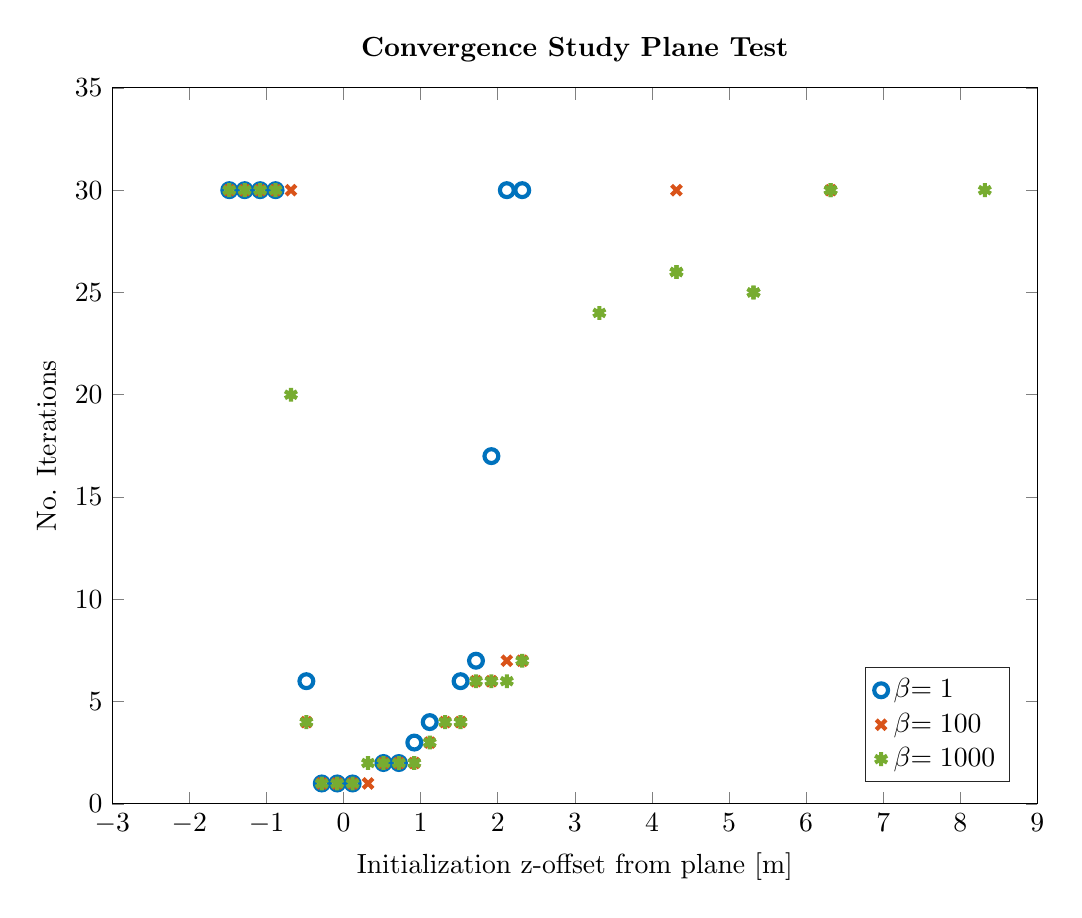
\begin{tikzpicture}

\begin{axis}[%
width=0.969\textwidth,
height=0.75\textwidth,
at={(0\textwidth,0\textwidth)},
scale only axis,
xmin=-3,
xmax=9,
xlabel={Initialization z-offset from plane [m]},
ymin=0,
ymax=35,
ylabel={No. Iterations},
axis background/.style={fill=white},
title style={font=\bfseries},
title={Convergence Study Plane Test},
legend style={at={(0.97,0.03)},anchor=south east,legend cell align=left,align=left,draw=white!15!black}
]
\addplot [color=mycolor1,line width=1.5pt,mark size=2.5pt,only marks,mark=o,mark options={solid}]
  table[row sep=crcr]{%
1.5178	6\\
1.1178	4\\
1.7178	7\\
0.9178	3\\
1.9178	17\\
0.7178	2\\
2.1178	30\\
0.5178	2\\
2.3178	30\\
0.1178	1\\
-0.8822	30\\
-0.0821999999999998	1\\
-1.0822	30\\
-0.2822	1\\
-1.2822	30\\
-0.4822	6\\
-1.4822	30\\
};
\addlegendentry{$\beta\text{ = 1}$};

\addplot [color=mycolor2,line width=1.5pt,mark size=2.5pt,only marks,mark=x,mark options={solid}]
  table[row sep=crcr]{%
21.3178	30\\
11.3178	30\\
6.3178	30\\
4.3178	30\\
1.3178	4\\
0.3178	1\\
-0.6822	30\\
2.3178	7\\
0.1178	1\\
-0.8822	30\\
-0.0821999999999998	1\\
-1.0822	30\\
-0.2822	1\\
-1.2822	30\\
-0.4822	4\\
-1.4822	30\\
1.5178	4\\
1.1178	3\\
1.7178	6\\
0.9178	2\\
1.9178	6\\
0.7178	2\\
2.1178	7\\
0.5178	2\\
};
\addlegendentry{$\beta\text{ = 100}$};

\addplot [color=mycolor3,line width=1.5pt,mark size=2.5pt,only marks,mark=asterisk,mark options={solid}]
  table[row sep=crcr] &
    \includegraphics[valign=b,width=.35\linewidth]{figures/planetest3d.png}\\
\end{tabular}
}

%\frame{\frametitle{Simulation test case}}
\frame{
  \frametitle{Middlebury dataset results}
  
  \begin{figure}[H]
  \begin{subfigure}{.2\linewidth}
    \includegraphics[width=\textwidth]{figures/recycle0.png}
  \end{subfigure}
  \begin{subfigure}{.2\linewidth}
    \includegraphics[width=\textwidth]{figures/middlebury_residuals_b1.png}
  \end{subfigure}
  \begin{subfigure}{.2\linewidth}
    \includegraphics[width=\textwidth]{figures/middlebury_residuals_b10.png}
  \end{subfigure}
  \end{figure}
  
  \begin{figure}[H]
  \begin{subfigure}{.2\linewidth}
    \includegraphics[width=\textwidth]{figures/middlebury_3d_groundtruth.png}
  \end{subfigure}
  \begin{subfigure}{.2\linewidth}
    \includegraphics[width=\textwidth]{figures/middlebury_3d_b1.png}
  \end{subfigure}
  \begin{subfigure}{.2\linewidth}
    \includegraphics[width=\textwidth]{figures/middlebury_3d_b10.png}
  \end{subfigure}
  \end{figure}
  
  \begin{figure}[H]
  \begin{subfigure}{.2\linewidth}
    \includegraphics[width=\textwidth]{figures/middlebury_disparity.png}
  \end{subfigure}
  \begin{subfigure}{.2\linewidth}
    \includegraphics[width=\textwidth]{figures/middlebury_disparity_b1.png}
  \end{subfigure}
  \begin{subfigure}{.2\linewidth}
    \includegraphics[width=\textwidth]{figures/middlebury_disparity_b10.png}
  \end{subfigure}
  \end{figure}

}

\frame{
  \frametitle{Middlebury dataset convergence}

\resizebox{\linewidth}{!}{
  % This file was created by matlab2tikz.
%
%The latest updates can be retrieved from
%  http://www.mathworks.com/matlabcentral/fileexchange/22022-matlab2tikz-matlab2tikz
%where you can also make suggestions and rate matlab2tikz.
%
\definecolor{mycolor1}{rgb}{0.00000,0.44700,0.74100}%
\definecolor{mycolor2}{rgb}{0.85000,0.32500,0.09800}%
\definecolor{mycolor3}{rgb}{0.46600,0.67400,0.18800}%
%
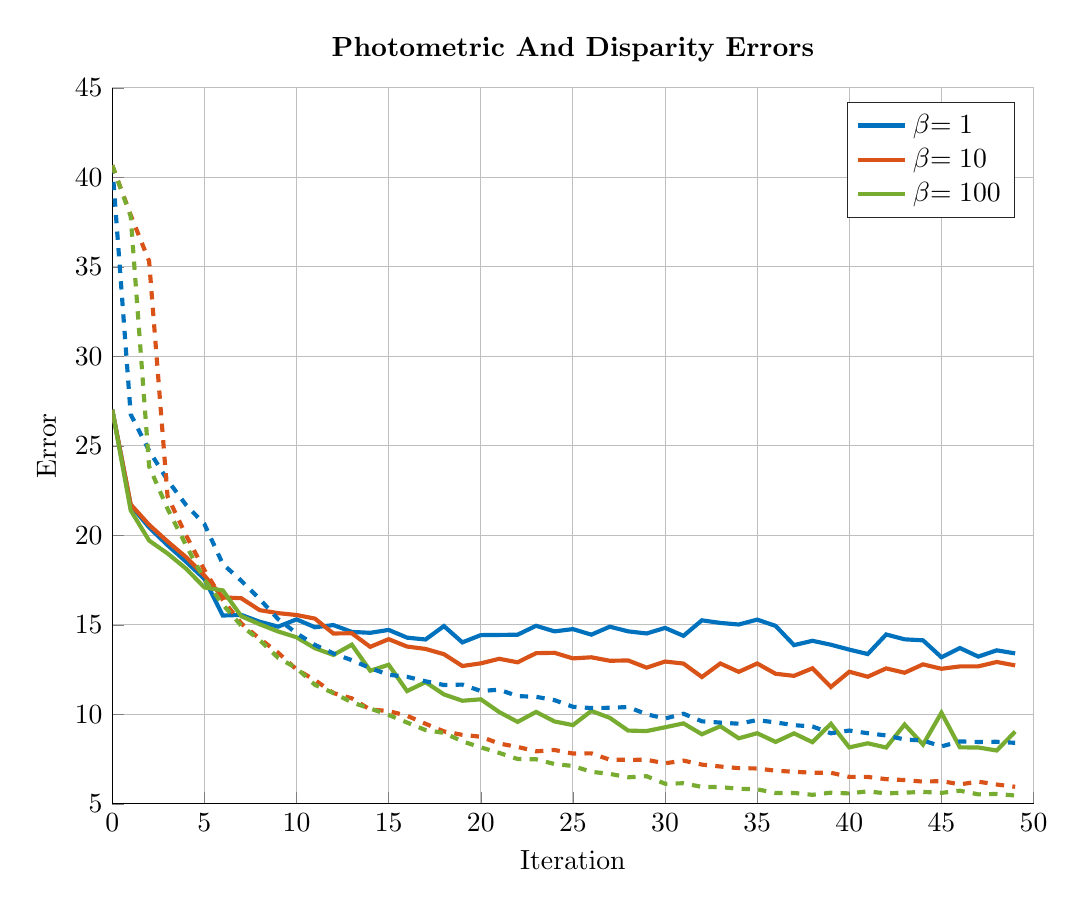
\begin{tikzpicture}

\begin{axis}[%
width=0.965\linewidth,
height=0.75\linewidth,
at={(0\linewidth,0\linewidth)},
scale only axis,
xmin=0,
xmax=50,
xlabel={Iteration},
xmajorgrids,
ymin=5,
ymax=45,
ylabel={Error},
ymajorgrids,
axis background/.style={fill=white},
title style={font=\bfseries},
title={Photometric And Disparity Errors},
axis x line*=bottom,
axis y line*=left,
legend style={legend cell align=left,align=left,draw=white!15!black}
]
\addplot [color=mycolor1,solid,line width=1.5pt]
  table[row sep=crcr]{%
0	27.0193\\
1	21.6862\\
2	20.4461\\
3	19.4545\\
4	18.5367\\
5	17.5694\\
6	15.5245\\
7	15.5588\\
8	15.1775\\
9	14.9028\\
10	15.3095\\
11	14.8702\\
12	14.9911\\
13	14.6092\\
14	14.5588\\
15	14.7201\\
16	14.2885\\
17	14.1852\\
18	14.9352\\
19	14.0251\\
20	14.4313\\
21	14.4402\\
22	14.4542\\
23	14.9513\\
24	14.6389\\
25	14.7659\\
26	14.4558\\
27	14.9008\\
28	14.6397\\
29	14.5226\\
30	14.8326\\
31	14.3902\\
32	15.2573\\
33	15.1115\\
34	15.0229\\
35	15.2958\\
36	14.9455\\
37	13.8706\\
38	14.1127\\
39	13.8935\\
40	13.6203\\
41	13.3731\\
42	14.4654\\
43	14.1949\\
44	14.139\\
45	13.1936\\
46	13.7095\\
47	13.2302\\
48	13.5807\\
49	13.4102\\
};
\addlegendentry{$\beta\text{ = 1}$};

\addplot [color=mycolor2,solid,line width=1.5pt]
  table[row sep=crcr]{%
0	27.0193\\
1	21.73\\
2	20.5923\\
3	19.6625\\
4	18.7929\\
5	17.7596\\
6	16.536\\
7	16.4912\\
8	15.825\\
9	15.6585\\
10	15.5537\\
11	15.3525\\
12	14.5206\\
13	14.5352\\
14	13.7747\\
15	14.2039\\
16	13.7912\\
17	13.659\\
18	13.3641\\
19	12.7051\\
20	12.8529\\
21	13.1074\\
22	12.9109\\
23	13.4215\\
24	13.4421\\
25	13.1302\\
26	13.1912\\
27	12.9979\\
28	13.0144\\
29	12.6122\\
30	12.9553\\
31	12.8404\\
32	12.089\\
33	12.8458\\
34	12.3777\\
35	12.845\\
36	12.2704\\
37	12.1547\\
38	12.5767\\
39	11.5344\\
40	12.3844\\
41	12.105\\
42	12.5715\\
43	12.3301\\
44	12.7958\\
45	12.5504\\
46	12.6817\\
47	12.6851\\
48	12.9296\\
49	12.7389\\
};
\addlegendentry{$\beta\text{ = 10}$};

\addplot [color=mycolor3,solid,line width=1.5pt]
  table[row sep=crcr]{%
0	27.0193\\
1	21.3973\\
2	19.7126\\
3	18.9925\\
4	18.1475\\
5	17.0934\\
6	16.9272\\
7	15.4866\\
8	15.0373\\
9	14.6342\\
10	14.3092\\
11	13.6984\\
12	13.3233\\
13	13.895\\
14	12.4404\\
15	12.7744\\
16	11.3049\\
17	11.8034\\
18	11.1176\\
19	10.764\\
20	10.8437\\
21	10.1325\\
22	9.58349\\
23	10.1397\\
24	9.60642\\
25	9.40317\\
26	10.196\\
27	9.80837\\
28	9.09636\\
29	9.07219\\
30	9.28145\\
31	9.49979\\
32	8.89135\\
33	9.34103\\
34	8.66664\\
35	8.94864\\
36	8.46589\\
37	8.94028\\
38	8.4496\\
39	9.47633\\
40	8.15745\\
41	8.38703\\
42	8.15075\\
43	9.43356\\
44	8.31474\\
45	10.0943\\
46	8.15957\\
47	8.15242\\
48	7.98454\\
49	9.03887\\
};
\addlegendentry{$\beta\text{ = 100}$};

\addplot [color=mycolor1,dashed,line width=1.5pt,forget plot]
  table[row sep=crcr]{%
0	40.675\\
1	26.7639\\
2	24.7353\\
3	23.0847\\
4	21.7035\\
5	20.6369\\
6	18.3988\\
7	17.4694\\
8	16.4452\\
9	15.3238\\
10	14.5376\\
11	13.882\\
12	13.4074\\
13	13.0302\\
14	12.5861\\
15	12.2169\\
16	12.1019\\
17	11.85\\
18	11.6453\\
19	11.6656\\
20	11.3102\\
21	11.381\\
22	11.024\\
23	10.9837\\
24	10.7982\\
25	10.4271\\
26	10.3565\\
27	10.3717\\
28	10.4116\\
29	10.009\\
30	9.77062\\
31	10.0382\\
32	9.61643\\
33	9.54363\\
34	9.48125\\
35	9.68392\\
36	9.55442\\
37	9.39967\\
38	9.3265\\
39	8.94677\\
40	9.10005\\
41	8.94952\\
42	8.82641\\
43	8.60106\\
44	8.54271\\
45	8.21291\\
46	8.49241\\
47	8.46204\\
48	8.47082\\
49	8.41357\\
};
\addplot [color=mycolor2,dashed,line width=1.5pt,forget plot]
  table[row sep=crcr]{%
0	40.675\\
1	37.8954\\
2	35.3239\\
3	22.1851\\
4	20.0126\\
5	18.0662\\
6	16.3997\\
7	15.0832\\
8	14.2318\\
9	13.4502\\
10	12.5147\\
11	11.9181\\
12	11.1957\\
13	10.8983\\
14	10.2749\\
15	10.188\\
16	9.92482\\
17	9.47906\\
18	9.05177\\
19	8.8597\\
20	8.75343\\
21	8.37333\\
22	8.18493\\
23	7.93817\\
24	8.0139\\
25	7.81288\\
26	7.82532\\
27	7.47156\\
28	7.46314\\
29	7.46497\\
30	7.2698\\
31	7.42052\\
32	7.19663\\
33	7.08981\\
34	7\\
35	6.98079\\
36	6.85659\\
37	6.7966\\
38	6.74465\\
39	6.74209\\
40	6.5107\\
41	6.50887\\
42	6.38449\\
43	6.33309\\
44	6.2462\\
45	6.27602\\
46	6.09347\\
47	6.24474\\
48	6.08487\\
49	5.95866\\
};
\addplot [color=mycolor3,dashed,line width=1.5pt,forget plot]
  table[row sep=crcr]{%
0	40.675\\
1	37.8275\\
2	23.8593\\
3	21.4902\\
4	19.4578\\
5	17.5303\\
6	16.143\\
7	14.9559\\
8	14.152\\
9	13.1604\\
10	12.5877\\
11	11.6519\\
12	11.1955\\
13	10.6748\\
14	10.3285\\
15	9.96927\\
16	9.54564\\
17	9.12713\\
18	8.96671\\
19	8.49698\\
20	8.15987\\
21	7.85001\\
22	7.51107\\
23	7.49442\\
24	7.22919\\
25	7.11926\\
26	6.79587\\
27	6.6788\\
28	6.48802\\
29	6.5482\\
30	6.12877\\
31	6.15511\\
32	5.9497\\
33	5.93964\\
34	5.84781\\
35	5.8191\\
36	5.61112\\
37	5.61387\\
38	5.50942\\
39	5.63033\\
40	5.58606\\
41	5.70349\\
42	5.58643\\
43	5.62886\\
44	5.6724\\
45	5.61752\\
46	5.73898\\
47	5.5343\\
48	5.55698\\
49	5.47137\\
};
\end{axis}
\end{tikzpicture}%
  % This file was created by matlab2tikz.
%
%The latest updates can be retrieved from
%  http://www.mathworks.com/matlabcentral/fileexchange/22022-matlab2tikz-matlab2tikz
%where you can also make suggestions and rate matlab2tikz.
%
\definecolor{mycolor1}{rgb}{0.00000,0.44700,0.74100}%
\definecolor{mycolor2}{rgb}{0.85000,0.32500,0.09800}%
\definecolor{mycolor3}{rgb}{0.46600,0.67400,0.18800}%
%
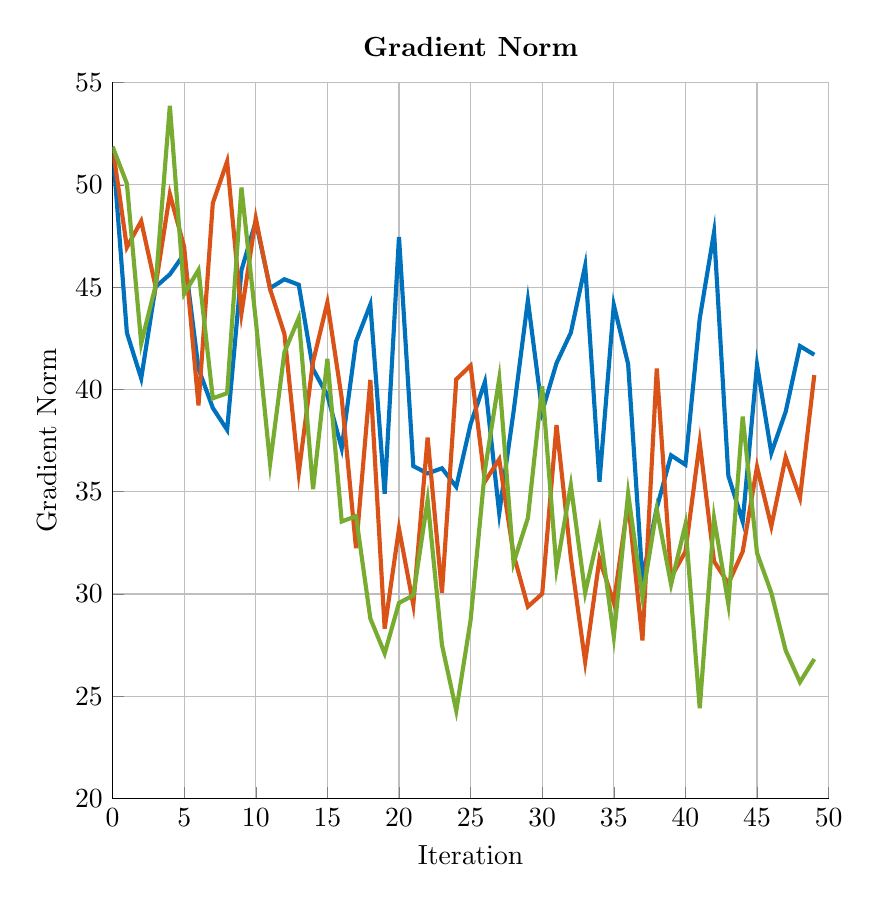
\begin{tikzpicture}

\begin{axis}[%
width=0.75\linewidth,
height=0.75\linewidth,
at={(0\linewidth,0\linewidth)},
scale only axis,
xmin=0,
xmax=50,
xlabel={Iteration},
xmajorgrids,
ymin=20,
ymax=55,
ylabel={Gradient Norm},
ymajorgrids,
axis background/.style={fill=white},
title style={font=\bfseries},
title={Gradient Norm},
axis x line*=bottom,
axis y line*=left
]
\addplot [color=mycolor1,solid,line width=1.5pt,forget plot]
  table[row sep=crcr]{%
0	51.8657333333333\\
1	42.7672\\
2	40.5361333333333\\
3	45.0064\\
4	45.62\\
5	46.6197333333333\\
6	41.0142666666667\\
7	39.0914666666667\\
8	38.0222666666667\\
9	45.8229333333333\\
10	48.2058666666667\\
11	44.9474666666667\\
12	45.3816\\
13	45.114\\
14	40.988\\
15	39.7074666666667\\
16	37.1174666666667\\
17	42.3354666666667\\
18	44.1462666666667\\
19	34.9008\\
20	47.4497333333333\\
21	36.2461333333333\\
22	35.8925333333333\\
23	36.1418666666667\\
24	35.2381333333333\\
25	38.3054666666667\\
26	40.3644\\
27	33.9444\\
28	38.9056\\
29	44.3508\\
30	38.9198666666667\\
31	41.2830666666667\\
32	42.7693333333333\\
33	46.0422666666667\\
34	35.4916\\
35	44.1261333333333\\
36	41.2369333333333\\
37	30.7421333333333\\
38	34.2036\\
39	36.7754666666667\\
40	36.3173333333333\\
41	43.4578666666667\\
42	47.6801333333333\\
43	35.7756\\
44	33.5366666666667\\
45	41.196\\
46	36.894\\
47	38.9030666666667\\
48	42.1165333333333\\
49	41.6921333333333\\
};
\addplot [color=mycolor2,solid,line width=1.5pt,forget plot]
  table[row sep=crcr]{%
0	51.8657333333333\\
1	46.9416\\
2	48.2238666666667\\
3	45.0296\\
4	49.5462666666667\\
5	46.9609333333333\\
6	39.2156\\
7	49.1041333333333\\
8	51.1397333333333\\
9	43.7181333333333\\
10	48.3673333333333\\
11	44.8945333333333\\
12	42.7089333333333\\
13	35.9128\\
14	41.3530666666667\\
15	44.2477333333333\\
16	39.5786666666667\\
17	32.2364\\
18	40.4630666666667\\
19	28.3054666666667\\
20	33.1944\\
21	29.4678666666667\\
22	37.6489333333333\\
23	30.0624\\
24	40.49\\
25	41.164\\
26	35.4932\\
27	36.5808\\
28	31.9290666666667\\
29	29.3802666666667\\
30	30.0101333333333\\
31	38.2597333333333\\
32	31.772\\
33	26.6877333333333\\
34	31.7098666666667\\
35	29.5690666666667\\
36	34.4930666666667\\
37	27.7288\\
38	41.0197333333333\\
39	30.8205333333333\\
40	32.0616\\
41	37.4044\\
42	31.5949333333333\\
43	30.5121333333333\\
44	32.0688\\
45	36.2146666666667\\
46	33.3098666666667\\
47	36.684\\
48	34.6953333333333\\
49	40.6966666666667\\
};
\addplot [color=mycolor3,solid,line width=1.5pt,forget plot]
  table[row sep=crcr]{%
0	51.8657333333333\\
1	50.0582666666667\\
2	42.2469333333333\\
3	45.0510666666667\\
4	53.8644\\
5	44.6676\\
6	45.8338666666667\\
7	39.5630666666667\\
8	39.8132\\
9	49.8693333333333\\
10	43.3732\\
11	36.3757333333333\\
12	41.8149333333333\\
13	43.49\\
14	35.1232\\
15	41.4886666666667\\
16	33.5413333333333\\
17	33.8029333333333\\
18	28.7984\\
19	27.0956\\
20	29.5616\\
21	29.9344\\
22	34.5862666666667\\
23	27.51\\
24	24.2962666666667\\
25	28.7162666666667\\
26	36.0522666666667\\
27	40.5266666666667\\
28	31.5210666666667\\
29	33.7089333333333\\
30	40.1468\\
31	31.2476\\
32	35.3134666666667\\
33	30.0609333333333\\
34	33.1505333333333\\
35	27.9064\\
36	34.9125333333333\\
37	29.8424\\
38	34.1369333333333\\
39	30.4633333333333\\
40	33.392\\
41	24.4152\\
42	33.7129333333333\\
43	29.4985333333333\\
44	38.6710666666667\\
45	32.0034666666667\\
46	30.0573333333333\\
47	27.2425333333333\\
48	25.694\\
49	26.8190666666667\\
};
\end{axis}
\end{tikzpicture}%
}
  
}

\frame{
  \frametitle{Inhouse dataset results}

  \scalebox{.9}{
    \begin{tabularx}{\textwidth}{Xr c c c}
      \footnotesize
  $\beta = 10$ \newline
  $\gamma = 1e5$
    &
    \multirow{2}{*}{
    \includegraphics[valign=t,width=.25\textwidth]{figures/bag_far_gt.png}
    } &
    \multirow{2}{*}{
    \includegraphics[valign=t,width=.25\textwidth]{figures/bag_far_map.png}
    } &
    \includegraphics[valign=t,width=.2\textwidth]{figures/disparity_map_far_hr.png} \\
    & & &
    \includegraphics[valign=t,width=.2\textwidth]{figures/disparity_gt_far.png} \\
      \footnotesize
  $\beta = 10$ \newline
  $\gamma = 1e5$ 
    & \multirow{2}{*}{
    \includegraphics[valign=t,width=.25\textwidth]{figures/bag_close_gt.png} 
    } &
    \multirow{2}{*}{
    \includegraphics[valign=t,width=.25\textwidth]{figures/bag_close_map.png} 
    } &
    \includegraphics[valign=t,width=.2\textwidth]{figures/disparity_map_close_hr.png} \\
    & & &
    \includegraphics[valign=t,width=.2\textwidth]{figures/disparity_gt_close.png} \\
  \end{tabularx}
}

}

\frame{
  \frametitle{Inhouse dataset convergence}
  \resizebox{\linewidth}{!}{
    % This file was created by matlab2tikz.
%
%The latest updates can be retrieved from
%  http://www.mathworks.com/matlabcentral/fileexchange/22022-matlab2tikz-matlab2tikz
%where you can also make suggestions and rate matlab2tikz.
%
\definecolor{mycolor1}{rgb}{0.00000,0.44700,0.74100}%
\definecolor{mycolor2}{rgb}{0.85000,0.32500,0.09800}%
\definecolor{mycolor3}{rgb}{0.46600,0.67400,0.18800}%
\definecolor{mycolor4}{rgb}{0.49400,0.18400,0.55600}%
%
\begin{tikzpicture}

\begin{axis}[%
width=0.969\linewidth,
height=0.75\linewidth,
at={(0\linewidth,0\linewidth)},
scale only axis,
xmin=0,
xmax=30,
xlabel={Iteration},
xmajorgrids,
ymin=0,
ylabel={Error},
ymajorgrids,
axis background/.style={fill=white},
title style={font=\bfseries},
title={Photometric RMSE},
axis x line*=bottom,
axis y line*=left,
legend style={legend cell align=left,align=left,draw=white!15!black}
]
\addplot [color=mycolor1,solid,line width=1.5pt]
  table[row sep=crcr]{%
0	32.8765\\
1	30.7613\\
2	28.4269\\
3	25.3259\\
4	22.539\\
5	19.3246\\
6	16.0249\\
7	14.4648\\
8	13.4227\\
9	13.3361\\
10	12.6765\\
11	12.4527\\
12	11.8476\\
13	12.0018\\
14	11.4839\\
15	11.5655\\
16	11.819\\
17	11.7148\\
18	11.8078\\
19	11.6447\\
20	12.0251\\
21	11.9872\\
22	11.7451\\
23	12.415\\
24	11.6159\\
25	11.6755\\
26	10.809\\
27	12.1347\\
28	11.6383\\
29	11.8771\\
};
\addlegendentry{Close};

\addplot [color=mycolor2,solid,line width=1.5pt]
  table[row sep=crcr]{%
0	32.8765\\
1	30.6668\\
2	28.5774\\
3	25.6998\\
4	23.0307\\
5	19.9675\\
6	16.7695\\
7	14.6451\\
8	12.8529\\
9	11.67\\
10	11.0326\\
11	10.672\\
12	10.1455\\
13	9.99341\\
14	9.87842\\
15	9.6155\\
16	9.07102\\
17	8.41648\\
18	8.0555\\
19	7.21861\\
20	7.35917\\
21	7.16422\\
22	7.0774\\
23	6.58987\\
24	6.75989\\
25	6.5806\\
26	6.52855\\
27	6.32808\\
28	6.49009\\
29	6.26694\\
};
\addlegendentry{$\text{Close with }\gamma$};

\addplot [color=mycolor3,solid,line width=1.5pt]
  table[row sep=crcr]{%
0	12.219\\
1	8.43807\\
2	5.75557\\
3	5.64414\\
4	5.06052\\
5	4.92199\\
6	4.48379\\
7	4.79279\\
8	4.79033\\
9	5.18879\\
10	5.39492\\
11	5.75986\\
12	5.96856\\
13	5.88106\\
14	5.86797\\
15	6.229\\
16	6.6267\\
17	6.59556\\
18	6.26931\\
19	6.77066\\
20	6.93361\\
21	5.9215\\
22	6.31606\\
23	6.02172\\
24	6.66415\\
25	6.85459\\
26	6.53181\\
27	6.71777\\
28	6.81212\\
29	6.13852\\
};
\addlegendentry{Far};

\addplot [color=mycolor4,solid,line width=1.5pt]
  table[row sep=crcr]{%
0	12.219\\
1	8.32782\\
2	5.63938\\
3	5.51586\\
4	5.07539\\
5	4.90134\\
6	4.32102\\
7	4.47033\\
8	4.48355\\
9	4.52778\\
10	4.46472\\
11	4.81814\\
12	4.61121\\
13	4.8298\\
14	4.53792\\
15	4.82781\\
16	4.74083\\
17	4.9326\\
18	4.66009\\
19	5.03098\\
20	4.79117\\
21	4.95051\\
22	4.87511\\
23	5.21122\\
24	4.95826\\
25	5.17446\\
26	5.02563\\
27	5.41652\\
28	5.20287\\
29	5.42374\\
};
\addlegendentry{$\text{Far with }\gamma$};

\addplot [color=mycolor1,dashed,line width=1.5pt,forget plot]
  table[row sep=crcr]{%
0	-1\\
1	-1\\
2	-1\\
3	-1\\
4	-1\\
5	-1\\
6	-1\\
7	-1\\
8	-1\\
9	-1\\
10	-1\\
11	-1\\
12	-1\\
13	-1\\
14	-1\\
15	-1\\
16	-1\\
17	-1\\
18	-1\\
19	-1\\
20	-1\\
21	-1\\
22	-1\\
23	-1\\
24	-1\\
25	-1\\
26	-1\\
27	-1\\
28	-1\\
29	-1\\
};
\addplot [color=mycolor2,dashed,line width=1.5pt,forget plot]
  table[row sep=crcr]{%
0	-1\\
1	-1\\
2	-1\\
3	-1\\
4	-1\\
5	-1\\
6	-1\\
7	-1\\
8	-1\\
9	-1\\
10	-1\\
11	-1\\
12	-1\\
13	-1\\
14	-1\\
15	-1\\
16	-1\\
17	-1\\
18	-1\\
19	-1\\
20	-1\\
21	-1\\
22	-1\\
23	-1\\
24	-1\\
25	-1\\
26	-1\\
27	-1\\
28	-1\\
29	-1\\
};
\addplot [color=mycolor3,dashed,line width=1.5pt,forget plot]
  table[row sep=crcr]{%
0	-1\\
1	-1\\
2	-1\\
3	-1\\
4	-1\\
5	-1\\
6	-1\\
7	-1\\
8	-1\\
9	-1\\
10	-1\\
11	-1\\
12	-1\\
13	-1\\
14	-1\\
15	-1\\
16	-1\\
17	-1\\
18	-1\\
19	-1\\
20	-1\\
21	-1\\
22	-1\\
23	-1\\
24	-1\\
25	-1\\
26	-1\\
27	-1\\
28	-1\\
29	-1\\
};
\addplot [color=mycolor4,dashed,line width=1.5pt,forget plot]
  table[row sep=crcr]{%
0	-1\\
1	-1\\
2	-1\\
3	-1\\
4	-1\\
5	-1\\
6	-1\\
7	-1\\
8	-1\\
9	-1\\
10	-1\\
11	-1\\
12	-1\\
13	-1\\
14	-1\\
15	-1\\
16	-1\\
17	-1\\
18	-1\\
19	-1\\
20	-1\\
21	-1\\
22	-1\\
23	-1\\
24	-1\\
25	-1\\
26	-1\\
27	-1\\
28	-1\\
29	-1\\
};
\end{axis}
\end{tikzpicture}%
    % This file was created by matlab2tikz.
%
%The latest updates can be retrieved from
%  http://www.mathworks.com/matlabcentral/fileexchange/22022-matlab2tikz-matlab2tikz
%where you can also make suggestions and rate matlab2tikz.
%
\definecolor{mycolor1}{rgb}{0.00000,0.44700,0.74100}%
\definecolor{mycolor2}{rgb}{0.85000,0.32500,0.09800}%
\definecolor{mycolor3}{rgb}{0.46600,0.67400,0.18800}%
\definecolor{mycolor4}{rgb}{0.49400,0.18400,0.55600}%
%
\begin{tikzpicture}

\begin{axis}[%
width=0.75\linewidth,
height=0.75\linewidth,
at={(0\linewidth,0\linewidth)},
scale only axis,
xmin=0,
xmax=30,
xlabel={Iteration},
xmajorgrids,
ymin=0,
ymax=50,
ylabel={Gradient Norm},
ymajorgrids,
axis background/.style={fill=white},
title style={font=\bfseries},
title={Gradient Norm},
axis x line*=bottom,
axis y line*=left
]
\addplot [color=mycolor1,solid,line width=1.5pt,forget plot]
  table[row sep=crcr]{%
0	28.0692\\
1	32.0008\\
2	34.4205333333333\\
3	38.2816\\
4	44.0072\\
5	46.7790666666667\\
6	35.8444\\
7	32.6792\\
8	27.1465333333333\\
9	25.9576\\
10	21.36\\
11	17.5892\\
12	16.7\\
13	19.9921333333333\\
14	15.2081333333333\\
15	18.5797333333333\\
16	17.368\\
17	20.0793333333333\\
18	19.072\\
19	20.5201333333333\\
20	16.8466666666667\\
21	17.0982666666667\\
22	17.6045333333333\\
23	18.3817333333333\\
24	17.4789333333333\\
25	16.7262666666667\\
26	16.8877333333333\\
27	18.3884\\
28	17.3121333333333\\
29	19.5434666666667\\
};
\addplot [color=mycolor2,solid,line width=1.5pt,forget plot]
  table[row sep=crcr]{%
0	28.0692\\
1	31.9670666666667\\
2	34.4009333333333\\
3	39.4426666666667\\
4	43.7588\\
5	43.0162666666667\\
6	37.2092\\
7	32.0392\\
8	30.1906666666667\\
9	24.9424\\
10	20.2328\\
11	18.8509333333333\\
12	15.3782666666667\\
13	14.498\\
14	15.4456\\
15	17.2182666666667\\
16	17.0093333333333\\
17	18.6292\\
18	14.6602666666667\\
19	12.4992533333333\\
20	13.4\\
21	12.67992\\
22	13.8892\\
23	10.8495733333333\\
24	10.6698533333333\\
25	9.936\\
26	8.79114666666667\\
27	9.79225333333333\\
28	9.64114666666667\\
29	10.2463466666667\\
};
\addplot [color=mycolor3,solid,line width=1.5pt,forget plot]
  table[row sep=crcr]{%
0	22.1426666666667\\
1	21.812\\
2	12.1117866666667\\
3	8.2276\\
4	6.64992\\
5	10.2033733333333\\
6	5.03486666666667\\
7	4.12789333333333\\
8	3.80101333333333\\
9	5.65546666666667\\
10	5.67774666666667\\
11	6.43896\\
12	5.67033333333333\\
13	6.21077333333333\\
14	5.5674\\
15	6.16214666666667\\
16	6.18482666666667\\
17	7.68502666666667\\
18	6.20497333333333\\
19	6.86\\
20	5.50704\\
21	6.64244\\
22	6.46972\\
23	5.68413333333333\\
24	6.32034666666667\\
25	7.51154666666667\\
26	6.82818666666667\\
27	7.29973333333333\\
28	5.85585333333333\\
29	6.75090666666667\\
};
\addplot [color=mycolor4,solid,line width=1.5pt,forget plot]
  table[row sep=crcr]{%
0	22.1426666666667\\
1	21.8341333333333\\
2	11.9432266666667\\
3	7.49733333333333\\
4	6.9146\\
5	9.90982666666667\\
6	3.90686666666667\\
7	2.90828\\
8	3.67957333333333\\
9	2.77857333333333\\
10	3.08748\\
11	3.76177333333333\\
12	4.12681333333333\\
13	4.02478666666667\\
14	3.44493333333333\\
15	3.91844\\
16	4.98645333333333\\
17	4.18917333333333\\
18	4.55374666666667\\
19	3.90125333333333\\
20	4.80889333333333\\
21	4.05044\\
22	4.95821333333333\\
23	4.42456\\
24	5.49065333333333\\
25	4.64897333333333\\
26	5.58512\\
27	7.4376\\
28	6.124\\
29	6.0902\\
};
\end{axis}
\end{tikzpicture}%
  }

}

\subsection{Localization}
\frame{
  \frametitle{Plane Test}

\resizebox{\linewidth}{!}{
  % This file was created by matlab2tikz.
%
%The latest updates can be retrieved from
%  http://www.mathworks.com/matlabcentral/fileexchange/22022-matlab2tikz-matlab2tikz
%where you can also make suggestions and rate matlab2tikz.
%
\definecolor{mycolor1}{rgb}{0.00000,0.44700,0.74100}%
\definecolor{mycolor2}{rgb}{0.85000,0.32500,0.09800}%
%
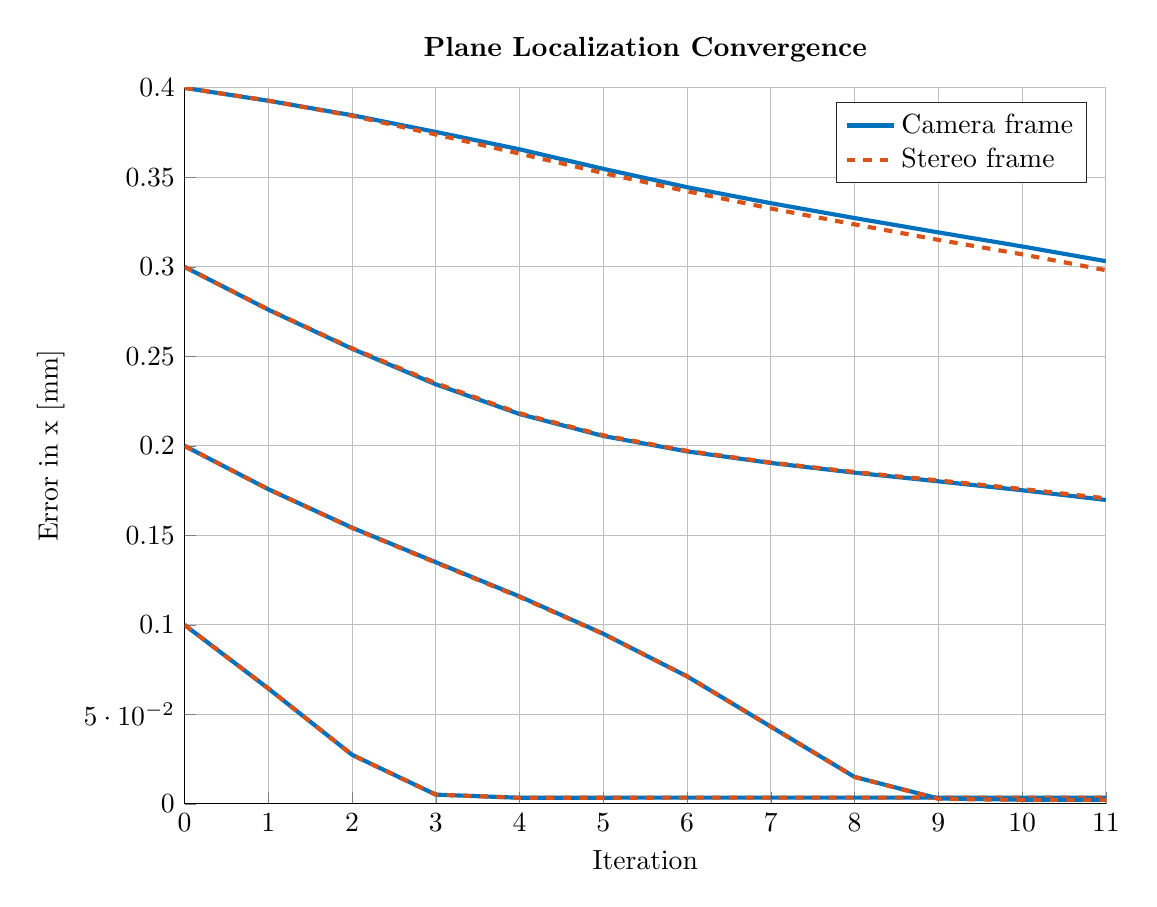
\begin{tikzpicture}

\begin{axis}[%
width=0.965\linewidth,
height=0.75\linewidth,
at={(0\linewidth,0\linewidth)},
scale only axis,
xmin=0,
xmax=11,
xlabel={Iteration},
xmajorgrids,
ymin=0,
ymax=0.4,
ylabel={Error in x [mm]},
ymajorgrids,
axis background/.style={fill=white},
title style={font=\bfseries},
title={Plane Localization Convergence},
axis x line*=bottom,
axis y line*=left,
legend style={legend cell align=left,align=left,draw=white!15!black}
]
\addplot [color=mycolor1,solid,line width=1.5pt]
  table[row sep=crcr]{%
0	0.1\\
1	0.0644761\\
2	0.0274531\\
3	0.00519103\\
4	0.0034475\\
5	0.00349513\\
6	0.0035024\\
7	0.00350495\\
8	0.00350593\\
9	0.00350651\\
10	0.00350698\\
11	0.00350743\\
};
\addlegendentry{Camera frame};

\addplot [color=mycolor2,dashed,line width=1.5pt]
  table[row sep=crcr]{%
0	0.1\\
1	0.0645072\\
2	0.0274247\\
3	0.00519983\\
4	0.00343936\\
5	0.00349233\\
6	0.0034978\\
7	0.00349912\\
8	0.00349971\\
9	0.00350017\\
10	0.00350062\\
11	0.00350106\\
};
\addlegendentry{Stereo frame};

\addplot [color=mycolor1,solid,line width=1.5pt,forget plot]
  table[row sep=crcr]{%
0	0.2\\
1	0.175815\\
2	0.154312\\
3	0.135028\\
4	0.115895\\
5	0.0950543\\
6	0.0712681\\
7	0.0431548\\
8	0.0150702\\
9	0.00302566\\
10	0.0023707\\
11	0.00230964\\
};
\addplot [color=mycolor1,solid,line width=1.5pt,forget plot]
  table[row sep=crcr]{%
0	0.3\\
1	0.276083\\
2	0.25427\\
3	0.234399\\
4	0.217788\\
5	0.205519\\
6	0.196912\\
7	0.190474\\
8	0.18505\\
9	0.180198\\
10	0.175237\\
11	0.169814\\
};
\addplot [color=mycolor1,solid,line width=1.5pt,forget plot]
  table[row sep=crcr]{%
0	0.4\\
1	0.392797\\
2	0.384716\\
3	0.375381\\
4	0.365675\\
5	0.354762\\
6	0.344509\\
7	0.335581\\
8	0.327275\\
9	0.319262\\
10	0.311429\\
11	0.303183\\
};
\addplot [color=mycolor2,dashed,line width=1.5pt,forget plot]
  table[row sep=crcr]{%
0	0.2\\
1	0.175858\\
2	0.154183\\
3	0.134775\\
4	0.115606\\
5	0.0949415\\
6	0.0712597\\
7	0.0431752\\
8	0.0150662\\
9	0.00283458\\
10	0.00227835\\
11	0.00228183\\
};
\addplot [color=mycolor2,dashed,line width=1.5pt,forget plot]
  table[row sep=crcr]{%
0	0.3\\
1	0.276188\\
2	0.254543\\
3	0.235021\\
4	0.218226\\
5	0.205923\\
6	0.197247\\
7	0.190702\\
8	0.185414\\
9	0.18071\\
10	0.175928\\
11	0.170697\\
};
\addplot [color=mycolor2,dashed,line width=1.5pt,forget plot]
  table[row sep=crcr]{%
0	0.4\\
1	0.392895\\
2	0.384405\\
3	0.373969\\
4	0.363267\\
5	0.352398\\
6	0.342248\\
7	0.33263\\
8	0.323737\\
9	0.315093\\
10	0.307018\\
11	0.298159\\
};
\end{axis}
\end{tikzpicture}%
  % This file was created by matlab2tikz.
%
%The latest updates can be retrieved from
%  http://www.mathworks.com/matlabcentral/fileexchange/22022-matlab2tikz-matlab2tikz
%where you can also make suggestions and rate matlab2tikz.
%
\definecolor{mycolor1}{rgb}{0.00000,0.44700,0.74100}%
\definecolor{mycolor2}{rgb}{0.85000,0.32500,0.09800}%
%
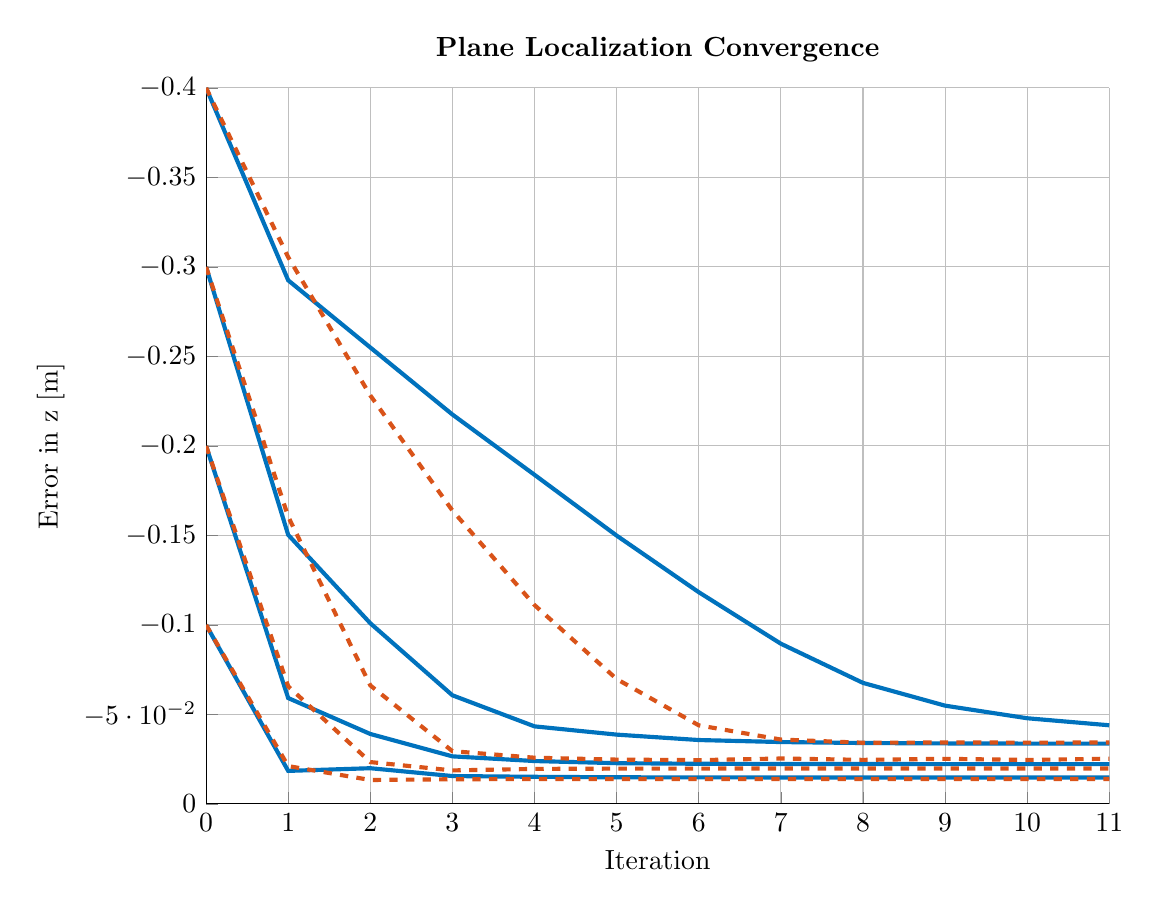
\begin{tikzpicture}

\begin{axis}[%
width=0.946\linewidth,
height=0.75\linewidth,
at={(0\linewidth,0\linewidth)},
scale only axis,
xmin=0,
xmax=11,
xlabel={Iteration},
xmajorgrids,
y dir=reverse,
ymin=-0.4,
ymax=0,
ylabel={Error in z [m]},
ymajorgrids,
axis background/.style={fill=white},
title style={font=\bfseries},
title={Plane Localization Convergence},
axis x line*=bottom,
axis y line*=left
]
\addplot [color=mycolor1,solid,line width=1.5pt,forget plot]
  table[row sep=crcr]{%
0	-0.1\\
1	-0.0184616\\
2	-0.0199583\\
3	-0.015583\\
4	-0.0151577\\
5	-0.0148843\\
6	-0.0148292\\
7	-0.0148084\\
8	-0.0148032\\
9	-0.0148016\\
10	-0.0148012\\
11	-0.0148012\\
};
\addplot [color=mycolor2,dashed,line width=1.5pt,forget plot]
  table[row sep=crcr]{%
0	-0.1\\
1	-0.0211318\\
2	-0.0133746\\
3	-0.0138027\\
4	-0.0138788\\
5	-0.0138921\\
6	-0.0138945\\
7	-0.013895\\
8	-0.0138952\\
9	-0.0138953\\
10	-0.0138954\\
11	-0.0138955\\
};
\addplot [color=mycolor1,solid,line width=1.5pt,forget plot]
  table[row sep=crcr]{%
0	-0.2\\
1	-0.0591501\\
2	-0.0390832\\
3	-0.0265814\\
4	-0.0239639\\
5	-0.022771\\
6	-0.0224403\\
7	-0.0223164\\
8	-0.0222779\\
9	-0.0222644\\
10	-0.02226\\
11	-0.0222584\\
};
\addplot [color=mycolor1,solid,line width=1.5pt,forget plot]
  table[row sep=crcr]{%
0	-0.3\\
1	-0.15031\\
2	-0.100936\\
3	-0.0606885\\
4	-0.043331\\
5	-0.0387217\\
6	-0.0357027\\
7	-0.0345741\\
8	-0.034033\\
9	-0.0338089\\
10	-0.0337098\\
11	-0.0336683\\
};
\addplot [color=mycolor1,solid,line width=1.5pt,forget plot]
  table[row sep=crcr]{%
0	-0.4\\
1	-0.292505\\
2	-0.254982\\
3	-0.217541\\
4	-0.183851\\
5	-0.149909\\
6	-0.118289\\
7	-0.0895129\\
8	-0.0676243\\
9	-0.0549032\\
10	-0.0478685\\
11	-0.0439413\\
};
\addplot [color=mycolor2,dashed,line width=1.5pt,forget plot]
  table[row sep=crcr]{%
0	-0.2\\
1	-0.065695\\
2	-0.0233879\\
3	-0.0187205\\
4	-0.0195734\\
5	-0.0197259\\
6	-0.0197549\\
7	-0.0197605\\
8	-0.0197615\\
9	-0.0197615\\
10	-0.0197614\\
11	-0.0197613\\
};
\addplot [color=mycolor2,dashed,line width=1.5pt,forget plot]
  table[row sep=crcr]{%
0	-0.3\\
1	-0.160484\\
2	-0.0662133\\
3	-0.0294704\\
4	-0.0258236\\
5	-0.0247636\\
6	-0.0244622\\
7	-0.0253769\\
8	-0.0246221\\
9	-0.0252002\\
10	-0.024578\\
11	-0.0252823\\
};
\addplot [color=mycolor2,dashed,line width=1.5pt,forget plot]
  table[row sep=crcr]{%
0	-0.4\\
1	-0.305453\\
2	-0.228196\\
3	-0.163903\\
4	-0.11109\\
5	-0.0697852\\
6	-0.0439192\\
7	-0.0359709\\
8	-0.0341758\\
9	-0.0343296\\
10	-0.0342604\\
11	-0.0343002\\
};
\end{axis}
\end{tikzpicture}%
}
}

%\frame{\frametitle{Simulation test case}}
